\chapter{Authentication in RFID protocol}

\section{Introduction}
    The chosen paper\cite{BOM}'s authentication is presented in the following chapter. The Protocol makes use of a diagonal block local transpose key matrix (DBLTKM) 
    encryption algorithm for it's property of 
    expanding the key size of the encryption without need of extensive resources. It insurres a balance between security and lightness of operations. 
    Another component is the self updating encryption 
    order (SUEO) and it's role is to boost security. Lastly a adaptive modulus (AM) algorithm is deployed to weaken the correlation between the 
    plaintext and the ciphertext.
    
    These three algorithms are used to form the block-order-modulus variable matrix encryption algorithm, dubbed the AM-SUEO-DBLTKM algorithm.

\section{Protocol's structure}

    \cite{BOM} proposes 3 corollaries based on block matrix properties and modulo operations that make the base for the primitives.

    A. \textbf{Diagonal block local transpose key matrix (DBLTKM)}

    For two square matrices $A_1$ and $A_2$: if $A_1 \times t_1$ mod(p) = $c_1$ and $A_2 \times t_2$ mod(p) = $c_2$ exist then:
    \begin{gather*}
        \begin{pmatrix}
        A_1 &  \\
            & A_2
        \end{pmatrix}
        \times
        \begin{pmatrix}
            t_1  \\
            t_2
        \end{pmatrix}
        mod(p)
        =
        \begin{pmatrix}
            c_1  \\
            c_2
        \end{pmatrix}
    \end{gather*}

    Updating the order of the first matrix along the main diagonal yields multiple key matrices of different sizes thus expanding the key size. For the fact that 
    it uses 2 matrices $A_1$ and $A_2$ as its building blocks the tag does not need to keep multiple separate keys in its memory. In order to expand the potential
    methods to build the key matrix, the transpose of $A_1$ and  of $A_2$ are also used as building blocks along the main diagonal.

    B. \textbf{Self updating encryption order (SUEO)}

    For 2 square matrices $A_1$ and $A_2$: if $A_1 \times t$ mod(p) = $c_1$ and $A_2 \times c_1$ mod(p) = $c_2$ exist and $A_2 \times t$ mod(p) = $c_3$ and 
    $A_1 \times c_3$ mod(p) = $c_4$ exist then: 
    
    \begin{gather*}
        c_2 \neq c_4
    \end{gather*}

    Using the property of non-commutativity of matrices, one can change the order of the multiplications to get different ciphertexts. This change is equivalent to having multiple keys for
    encryption but with this result security can be improved without using additional storage space.

    C. \textbf{Adaptive modulus (AM)}

    For 2 square matrices $A$ and $B$ and $A \times B$ = $I$(identity matrix)mod(p) then: 
    
    \begin{gather*}
        \textit{B is the modulus p-inverse matrix of A and the modulus q-inverse of A,}\\
        \textit{for a q integer divisor of p.}
    \end{gather*}

    Thus the change in modulus still yields an inverse and the decryption process can still happen but the correlation between the ciphertext and the plaintext is weakened.

    D. \textbf{DBKM-SUEO-SUM}

    The above three components can be used for an encryption and decryption algorithm. The following figure represents an example with two key matrices and three
    integer divisors of modulus p.

    \begin{center}
    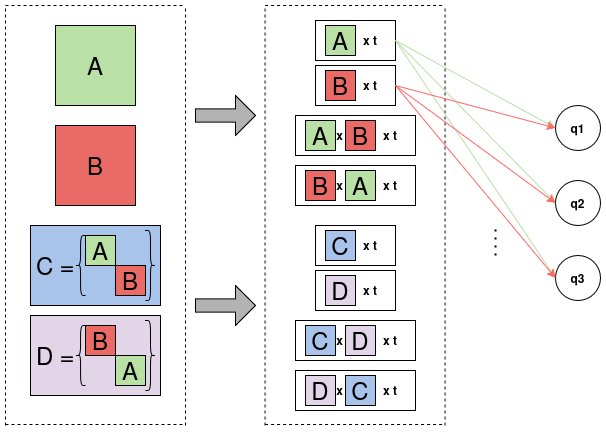
\includegraphics[width=0.7\textwidth]{Protocol_base_scheme.png}
    \end{center}

\section{Specific steps of the authentication protocol}

\begin{table}[H]
    \centering
    \caption{Notation used in the description of the protocol}
    \begin{tabular}{| c | c |}
        \hline
        Notation & Meaning \\
        \hline
        $N_t$ & Nonce generated by the tag \\
        $N_r$ & Nonce generated by the reader \\
        $S$ & Secret value \\
        $S_d$ & Secret value that determines the construction of the block key matrix  \\
        $S_p$ & Secret value that determines the encryption order  \\
        $S_c$ & Secret value that determines the selection of modulus  \\
        $p$ & Modulus  \\
        $q$ & q $\in$ f(p), f(p) is the set of integer divisors of p \\
        $N$ &  Total number of key matrices \\
        $Z_{DBLTKM}$ &  Total number of elements in the DBLTKM index table \\
        $Z_{SUEO}$ & Total number of elements in the SUEO index table  \\
        $Z_{AM}$ & Total number of elements in the AM index table  \\
        $A, A_{new}$ & Initial and updated encryption matrices \\
        $B, B_{new}$ & Initial and updated decryption matrices \\
        \hline
    \end{tabular}
\end{table}

\noindent{
    The notation used in the protocol are shown in table 1. The details of it are are follows:

    1. The reader sends a query to the tag. This activates tags without batteries.

    2. The tag uses its internal pseudo-random number generator to get nonce $N_t$. After that the tag uses the encryption matrix A and the modulus p to 
    encrypt $N_t||S$.

    3. The tag sends the message E($N_t||S$, A, p) to the reader. 

    4. The reader decrypts E($N_t||S$, A, p) and obtains the secret S. If S can be found in its internal database, the reader has authenticated the tag succesfully and accepted nonce $N_t$, else the protocol is stopped. 
        After that, the reader generates nonce $N_r$ and uses $A$ and $p$ to encrypt $N_r||S$. 

    5. The reader sends E($N_r||S$, A, p) to the server. 

    6. The server decrypts E($N_r||S$, A, p) and obtains secret S. A query on S suggests a succesfull authentication of the reader in which case the server accepts $N_r$. Contrarily the protocol is stopped.
        The server generates the new secret values $S_d, S_p, S_c$ and uses $A$ and $p$ to encrypt $N_r||S_d||S_p||S_c$.

    7. The server sends E($N_r||S_d||S_p||S_c$, A, p) to the reader. 

    8. The reader decrypts E($N_r||S_d||S_p||S_c$, A, p) and obtains $N_r$. If the received value $N_r$ matches the saved value $N_r$ then the reader authenticates 
    the server. In this case the new secret values 
        $S_d,S_p,S_c$ are accepted, if not the protocol is stopped. Afterwards the reader uses A and p to encrypt $N_t||S_d||S_p||S_c$. 

    9. The reader sends E($N_t||S_d||S_p||S_c$, A, p) to the tag. 

    10. The tag decrypts E($N_t||S_d||S_p||S_c$, A, p) and obtains $N_t$. If the value $N_t$ received matches the saved value $N_t$ then the tag authenticates the reader. Following that the new secret values 
        $S_d,S_p,S_c$ are accepted, if not the protocol is stopped. Subsequently fresh protocol parameters are calculted: mod($S_d, Z_{DBLTKM}$) to determine the construction of diagonal block key matrix, 
        mod($S_p, Z_{SUEO}$) to determine the encryption order, mod($S_c, Z_{AM}$) to determine the choice of the new modulus. With the newly constructed key matrix $A_{new}$, new modulus $q$ and encryption order, the tag 
        encrypts $N_t+1||ID$.

    11. The tag sends E($N_t+1||ID$, $A_{new}$, q) to the reader.
    
    12. Reader calculates mod($S_d, Z_{DBLTKM}$), mod($S_p, Z_{SUEO}$), mod($S_c, Z_{AM}$) itself. Then it decrypts E($N_t+1||ID$,$A_{new}$,q) 
    using the newly calculted $B_{new}$ and q. If the received value $N_t$ matches the saved value $N_t$, ID is obtained. The reader uses $A_{new}$ and q to encrypt $N_r+1||ID$. 

    13. The reader sends E($N_r+1||ID$, $A_{new}$, $q$) to the server.

    14. Server calculates mod($S_d, Z_{DBLTKM}$), mod($S_p, Z_{SUEO}$), mod($S_c, Z_{AM}$) itself. It decrypts E($N_r+1||ID$, $A_{new}$, $q$) using the newly calculted $B_{new}$ and q. If the received value $N_r$ 
    matches the saved value $N_r$, the server obtains ID.
    
}

% \newgeometry{left=1cm}

\begin{adjustwidth}{-30pt}{}
\procedureblock[colspace=-1cm]{The two way AM-SUEO-DBLTKM-RFID authentication protocol}{
    \textbf{Server} \< \< \textbf{Reader} \< \< \textbf{Tag} \\[-1ex]
    \textit{\footnotesize $A, B, p, S$} \< \< \textit{\footnotesize $A, B, p, S, N_r$} \< \< \textit{\footnotesize $A, B, p, S, N_t$} \\[-2ex]
    \textit{\footnotesize $Z_{DBLTKM}, Z_{SUEO}, Z_{AM}$} \< \< \textit{\footnotesize $Z_{DBLTKM}, Z_{SUEO}, Z_{AM}$} \< \< \textit{\footnotesize $Z_{DBLTKM}, Z_{SUEO}, Z_{AM}$} \\[-1.5ex]
    % \\
    \< \< \<\sendmessageright{top=\text{ \scriptsize 1.Query}} \< \\[-2ex]
    % \\
    \< \< \< \< \text{ \scriptsize 2.Generates $N_t$} \\[-2ex]
    \< \< \< \< \text{ \scriptsize E($N_t||S$, A, p)} \\[-3ex]
    % \\
    \< \< \< \sendmessageleft{top=\text{ \scriptsize 3.E($N_t||S$, A, p)}} \< \\[-4ex]
    % \\
    \< \< \text{ \scriptsize 4.D(E($N_t||S$, A, p), B, p)} \< \< \\[-2ex]
    \< \< \text{ \scriptsize Generates $N_r$} \< \< \\[-2ex]
    \< \< \text{ \scriptsize E($N_r||S$,A,p)} \< \< \\[-3ex]
    % \\
    \< \sendmessageleft{top=\text{ \scriptsize 5.E($N_r||S$, A, p)}} \< \< \< \\[-4ex]
    % \\
    \text{ \scriptsize 6.D(E($N_r||S$, A, p), B, p)} \< \< \< \< \\[-2ex]
    \text{ \scriptsize Generates $S_d, S_p, S_c$} \< \< \< \< \\[-2ex]
    \text{ \scriptsize E($N_r||S_d||S_p||S_c$, A, p)} \< \< \< \< \\[-4ex]
    % \\
    \< \sendmessageright{top = \text{ \scriptsize 7.E($N_r||S_d||S_p||S_c$, A, p)}} \< \< \< \\[-2ex]
    % \\
    \< \< \text{ \scriptsize 8.D(E($N_r||S_d||S_p||S_c$, A, p), B, p)} \< \< \\[-2ex]
    \< \< \text{ \scriptsize E($N_t||S_d||S_p||S_c$, A, p)} \< \< \\[-4ex]
    % \\
    \<\<\<\sendmessageright{top = \text{ \scriptsize 9.E($N_t||S_d||S_p||S_c$, A, p)}}\<\\[-2ex]
    % \\
    \< \< \< \< \text{ \scriptsize 10.D(E($N_t||S_d||S_p||S_c$, A, p), B, p)} \\[-2ex]
    \< \< \< \< \text{ \scriptsize Calculates mod($S_d, Z_{DBLTKM}$)} \\[-2ex]
    \< \< \< \< \text{ \scriptsize Calculates mod($S_p, Z_{SUEO}$)} \\[-2ex]
    \< \< \< \< \text{ \scriptsize Calculates mod($S_c, Z_{AM}$)} \\[-2ex]
    \< \< \< \< \text{ \scriptsize E($N_t+1||ID$, $A_{new}$, q)} \\[-2ex]
    % \\
    \< \< \< \sendmessageleft{top=\text{ \scriptsize 11.E($N_t+1||ID$, $A_{new}$, $q$)}} \< \\[-2ex]
    % \\
    \< \< \text{ \scriptsize 12.Calculates mod($S_d, Z_{DBLTKM}$)} \< \<\\[-2ex]
    \< \< \text{ \scriptsize Calculates mod($S_p, Z_{SUEO}$)} \< \<\\[-2ex]
    \< \< \text{ \scriptsize Calculates mod($S_c, Z_{AM}$)} \< \<\\[-2ex]
    \< \< \text{ \scriptsize D(E($N_t+1||ID$,$A_{new}$,$q$), $B_{new}$, $q$)} \< \<\\[-2ex]
    \< \< \text{ \scriptsize E($N_r+1||ID$, $A_{new}$, $q$)} \< \<\\[-1ex]
    % \\
    \< \sendmessageleft{top=\text{ \scriptsize 13.E($N_r+1||ID$, $A_{new}$, $q$)}} \< \< \< \\[-2ex]
    % \\
    \text{ \scriptsize 14.Calculates mod($S_d, Z_{DBLTKM}$)} \< \< \< \<\\[-2ex]
    \text{ \scriptsize Calculates mod($S_p, Z_{SUEO}$)} \< \< \< \<\\[-2ex]
    \text{ \scriptsize Calculates mod($S_c, Z_{AM}$)} \< \< \< \<\\[-2ex]
    \text{ \scriptsize D(E($N_r+1||ID$, $A_{new}$, $q$),} \< \< \< \<\\[-2ex]
    \text{ \scriptsize \ \ \ \ \ \ \ \ $B_{new}$, $q$)} \< \< \< \<\\[-2ex]
    \text{ \scriptsize Obtains ID} \< \< \< \<\\[-1ex]
}
\end{adjustwidth}
    
% \restoregeometry